\chapter{Graphics Library}

The graphics library is a library for making easy graphical objects in python. It was written by John Zelle for use with his book Python Programming: An
Introduction to Computer Science. This chapter is going to discuss the topics we covered during class. To use the library you have to import it first. For an explanation on how to import libraries see the section of the book.

\section{Creating a basic window}
The graphics library works as a programm of it own. A window gets updated as long as it gets changed or is waiting for a new command.
To draw somthing on a window we first have to create a window. A creation follows this pattern:
\begin{fullwidth}
\begin{python}
Window = GraphWin(WindowName, Width, Height)
Window.setCoords(StartX,StartY,WidthPixel,HeightPixel)
\end{python}
\end{fullwidth}

\section{Drawing on windows}
Now that we know how to create a window we can start drawing on it. There are various objects we can draw on windows. Because the graphics library uses its own coordinates system we need to use it for creating objects.
\begin{python}
Point(2,4) #Creates a point at 2,4
\end{python}
To actually draw in windows we have to use the draw command. 
\begin{fullwidth}
\begin{python}
Window = GraphWin(WindowName, Width, Height)
Window.setCoords(StartX,StartY,WidthPixel,HeightPixel)
Obj = OurObject
Obj.draw(Window)
\end{python}
\end{fullwidth}

In this example we are drawing Obj to our window.

\subsection{Rectangles}
In python rectangles are drawn from the down left point to the top right point.
\begin{python}
Rect = Rectangle(Point(X1,Y1),Point(X2,Y2))
\end{python}
This creates a rectangle calles Rect at the position X1 and Y1 with the width X2 and height Y2. 
After you have created your basic reactangle you can also color it.
\begin{fullwidth}
\begin{python}
Rect = Rectangle(Point(X1,Y1),Point(X2,Y2))
Rect.setFill(color_rgb(255,0,0)) #Set the color for the reactangle
\end{python}
\end{fullwidth}
\subsection{Circles}
Of course you can also add circles to your window. Circles are drawn from their middle point to the setting of the size of their diameter.
\begin{python}
C = Circle(Point(X,Y),Point(RX,RY))
\end{python}
The Point(X,Y) is defining the position of the circle. The Point(RX,RY) is defining the radius of the circle.

\subsection{Text labels}
On a window it is very important to be able to use text. Because of that the graphics library also comes with a text object for windows.
\begin{python}
T = Text(Point(X,Y),StringText)
\end{python}
The example is self explaining. But this text is nothing special. To make it cool we need to modifie it a bit.
\begin{fullwidth}
\begin{python}
Text.setFace(Font)
 #Availible Fonts are 'helvetica','arial','courier','times roman'
Text.setSize(Size) #Size of the text
Text.setStyle(Style)
 #Availible styles 'bold','normal','italic', 'bold italic'
Text.setTextColor(Color) # Use color_rgb(r,g,b) as a color
\end{python}
\end{fullwidth}

\newpage
\subsection{Other usefull methods}
There are some other usefull methods for the graphics library. Obj can be any object of the graphics library.
\begin{fullwidth}
\begin{python}
Obj.setFill(Color) #Sets the color
Obj.clone() #Creates a new object with the same properties as Obj.
Obj.move(X,Y) #Moves the object
color_rgb(r,g,b) #Makes a color for use with this library
Window.getMouse() #Stops the programm until you press on the screen
\end{python}
\end{fullwidth}

\subsection{Example code}
This is an example code of the graphics library.

\begin{marginfigure}[170pt]
  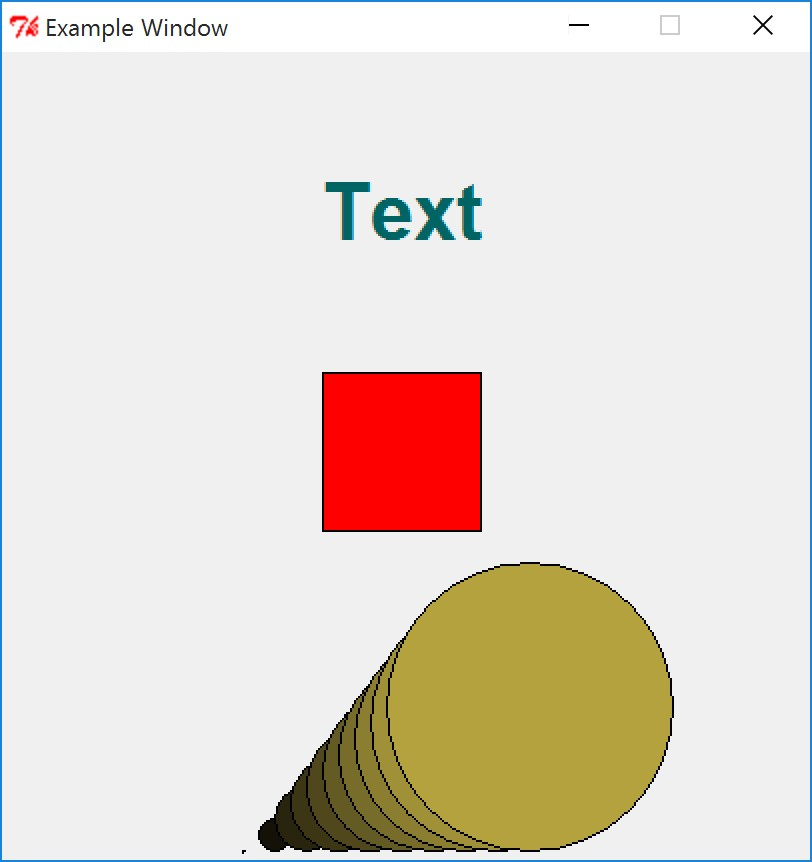
\includegraphics[width=\linewidth]{GraphicsExample1.jpg}
\end{marginfigure}
\begin{python}
from graphics import *

Win = GraphWin("Example Window",400,400)
Win.setCoords(0,0,50,50)
T = Text(Point(25,40), "Text")
T.draw(Win)
T.setFill(color_rgb(0,100,100))
T.setStyle("bold")
T.setFace("arial")
T.setSize(30)

Rect = Rectangle(Point(20,20),Point(30,30))
Rect.draw(Win)
Rect.setFill(color_rgb(255,0,0))

for i in range(10):
    C = Circle(Point(15+i*2,i),i)
    C.draw(Win)
    C.setFill(color_rgb(20*i,18*i,7*i))
\end{python}


















